%http://cs.pugetsound.edu/~jross/courses/cs240/project/requirements/
%Animation Group
\documentclass[12pt]{article}
\usepackage{titlesec}
\usepackage{graphicx}
\usepackage[labelformat=empty]{caption}
\titleformat{\section}[block]{\bfseries}{\thesection.}{1em}{} 
\titleformat{\subsection}[block]{\hspace{2em}}{\thesubsection}{1em}{}
\titleformat{\subsubsection}[block]{\hspace{2em}}{\subsubsection}{1em}{}
\titleformat{\paragraph}[block]{\hspace{5em}}{\paragraph}{6em}{}
\def\changemargin#1#2{\list{}{\rightmargin#2\leftmargin#1}\item[]}
\let\endchangemargin=\endlist 
%\setlength{\parindent}{4cm} % Default is 15pt.

\begin{document}

% Front Page
\begin{titlepage}
	\begin{center}
	\huge  Edith \\
	\vspace*{\fill}%
 	\huge \textbf{Animation System \\Final Report}
	\bigskip 
	\rule{130mm}{.1pt}
	\textsc{\textbf{December 7, 2013} \\ }
	\vspace*{\fill}%
	Eric Lund \\
	Kramer Canfield \\ 
	Zeke Rosenberg \\
	Calder Whiteley \\
	Jon Youmans
	\end{center}
\end{titlepage}

\section{\emph{Project Summary}}%Create a section for the introduction
\subsection{Edith System}
\begin{changemargin}{1cm}{0cm} 
This should be about the edith system This should be about the edith system This should be about the edith system This should be about the edith system This should be about the edith system This should be about the edith system This should be about the edith system This should be about the edith system This should be about the edith system This should be about the edith system This should be about the edith system This should be about the edith system This should be about the edith system This should be about the edith system This should be about the edith system This should be about the edith system This should be about the edith system This should be about the edith system This should be about the edith system This should be about the edith system This should be about the edith system This should be about the edith system This should be about the edith system This should be about the edith system This should be about the edith system This should be about the edith system This should be about the edith system This should be about the edith system This should be about the edith system This should be about the edith system
\end{changemargin} 
\subsection{Edith System}
\begin{changemargin}{1cm}{0cm} 
This should be about the animation system This should be about the animation system This should be about the animation system This should be about the animation system This should be about the animation system This should be about the animation system This should be about the animation system This should be about the animation system This should be about the animation system This should be about the animation system This should be about the animation system This should be about the animation system This should be about the animation system This should be about the animation system This should be about the animation system This should be about the animation system This should be about the animation system This should be about the animation system This should be about the animation system This should be about the animation system This should be about the animation system This should be about the animation system This should be about the animation system This should be about the animation system This should be about the animation system This should be about the animation system This should be about the animation system This should be about the animation system This should be about the animation system This should be about the animation system
\end{changemargin} 

\section{\emph{Development Procedures}}
In this section, provide a brief discussion of your development process. Your goal is to explain your development and evaluate what worked and what didn't. You should be sure and address the following points:

What kind of process model did you follow? (Likely this is a hybrid of multiple models we discussed in class). What components did you work on in what order? What was effective and not effective about your process and how you structured your development?
What forms of testing did you include? How do you know if your program works? What forms of testing were effective or ineffective?
Which team members were responsible for which components? This should be more than "everyone worked on everything"--who contributed what to the system?
Be sure and address all parts of the questions.

Include plenty of specifics in your descrption. This section should basically explain what you did in the course in terms of the final project, with enough detail that a reader could understand what activities you did and how you spent your time. Imagine writing for someone who hadn't taken the course and was curious what you did.
A key part of this discussion is analyzing what worked and what didn't. Be sure and address why you think some part of the process model wasn't effecive for this project. For example: why or why didn't putting together a requirements document help?
This section will likely be between 1 and 3 pages in length.\\ 

In this section, provide a brief discussion of your development process. Your goal is to explain your development and evaluate what worked and what didn't. You should be sure and address the following points:

What kind of process model did you follow? (Likely this is a hybrid of multiple models we discussed in class). What components did you work on in what order? What was effective and not effective about your process and how you structured your development?
What forms of testing did you include? How do you know if your program works? What forms of testing were effective or ineffective?
Which team members were responsible for which components? This should be more than "everyone worked on everything"--who contributed what to the system?
Be sure and address all parts of the questions.

Include plenty of specifics in your descrption. This section should basically explain what you did in the course in terms of the final project, with enough detail that a reader could understand what activities you did and how you spent your time. Imagine writing for someone who hadn't taken the course and was curious what you did.
A key part of this discussion is analyzing what worked and what didn't. Be sure and address why you think some part of the process model wasn't effecive for this project. For example: why or why didn't putting together a requirements document help?
This section will likely be between 1 and 3 pages in length.\\ 

In this section, provide a brief discussion of your development process. Your goal is to explain your development and evaluate what worked and what didn't. You should be sure and address the following points:

What kind of process model did you follow? (Likely this is a hybrid of multiple models we discussed in class). What components did you work on in what order? What was effective and not effective about your process and how you structured your development?
What forms of testing did you include? How do you know if your program works? What forms of testing were effective or ineffective?
Which team members were responsible for which components? This should be more than "everyone worked on everything"--who contributed what to the system?
Be sure and address all parts of the questions.

Include plenty of specifics in your descrption. This section should basically explain what you did in the course in terms of the final project, with enough detail that a reader could understand what activities you did and how you spent your time. Imagine writing for someone who hadn't taken the course and was curious what you did.
A key part of this discussion is analyzing what worked and what didn't. Be sure and address why you think some part of the process model wasn't effecive for this project. For example: why or why didn't putting together a requirements document help?
This section will likely be between 1 and 3 pages in length.\\ 

In this section, provide a brief discussion of your development process. Your goal is to explain your development and evaluate what worked and what didn't. You should be sure and address the following points:

What kind of process model did you follow? (Likely this is a hybrid of multiple models we discussed in class). What components did you work on in what order? What was effective and not effective about your process and how you structured your development?
What forms of testing did you include? How do you know if your program works? What forms of testing were effective or ineffective?
Which team members were responsible for which components? This should be more than "everyone worked on everything"--who contributed what to the system?
Be sure and address all parts of the questions.

Include plenty of specifics in your descrption. This section should basically explain what you did in the course in terms of the final project, with enough detail that a reader could understand what activities you did and how you spent your time. Imagine writing for someone who hadn't taken the course and was curious what you did.
A key part of this discussion is analyzing what worked and what didn't. Be sure and address why you think some part of the process model wasn't effecive for this project. For example: why or why didn't putting together a requirements document help?
This section will likely be between 1 and 3 pages in length.\\ 


\section{\emph{Requirements Evaluation}}
\section{\emph{System Design} \& \emph{Architecture}}
Animation teams final implementation is contained within one javascript file and contains a list of functions that can be utilized by other groups. These functions are primarily functions that animate objects (sprites) on the canvas but also include a few functions that allows for the ability to add sprites onto the canvas. To achieve this, our design utilizes and relies heavily on an external library called oCanvas. oCanvas is a JavaScript library that is intended to make development with a HTML5 Canvas easier. Instead of working with pixels, oCanvas allows for an object oriented interface allowing animations to be applied to objects, in our case, sprites. oCanvas can be thought of as strapping extra functionality onto a preexisting HTML5 canvas as all of the generic HTML5 canvas functions are still available and can be interweaved with any of the oCanvas functions. More information and documentation about oCanvas can be be found at their website: http://ocanvas.org. Because our code contained in one JavaScript file, we have appended the oCanvas library directly into our code as it can not be imported in line as it could be with HTML. \\

In order to begin using the animation functions the user needs to create a HTML5 canvas and assign it an ID. This ID can then be fed into our function called wrapHTMLCanvasToOcanvas(HTML5canvasID, background) which takes the HTML5 ID and a background color. This function simply takes the HTML5 canvas ID and calls the oCanvas function create() which creates the oCanvas. Our method then returns that oCanvas object. As stated above, this methods basically extends the HTML5 canvas adding more functionality to it -- it does not actually create a new canvas. After attaining the oCanvas object, sprites can then be added by calling the function addSprite(theOCanvas, image, width, height, xcoord, ycoord). The first parameter to this method is the oCanvas object which is returned from the first function wrapHTMLCanvasToOcanvas. The image parameter is a string of an image path to the image to be represented as the sprite. The remaining parameters deal with the size and location of the sprite. Once those steps have been completed the user can then animate the sprite using any of our animation functions. \\

This process can be simplified to a series of 4 steps:
\begin{itemize}
\item Create HTML5 canvas assigning it an ID.
\item wrapHTMLCanvasToOcanvas() to attain an oCanvas object.
\item Add sprites by calling addSprite().
\item Animate the sprites with the provided animation functions.\\
\end{itemize}

Below is a System state diagram that shows a sample implementation.\\

\begin{figure}
\caption{Figure 1. System State Diagram}
  \centering
    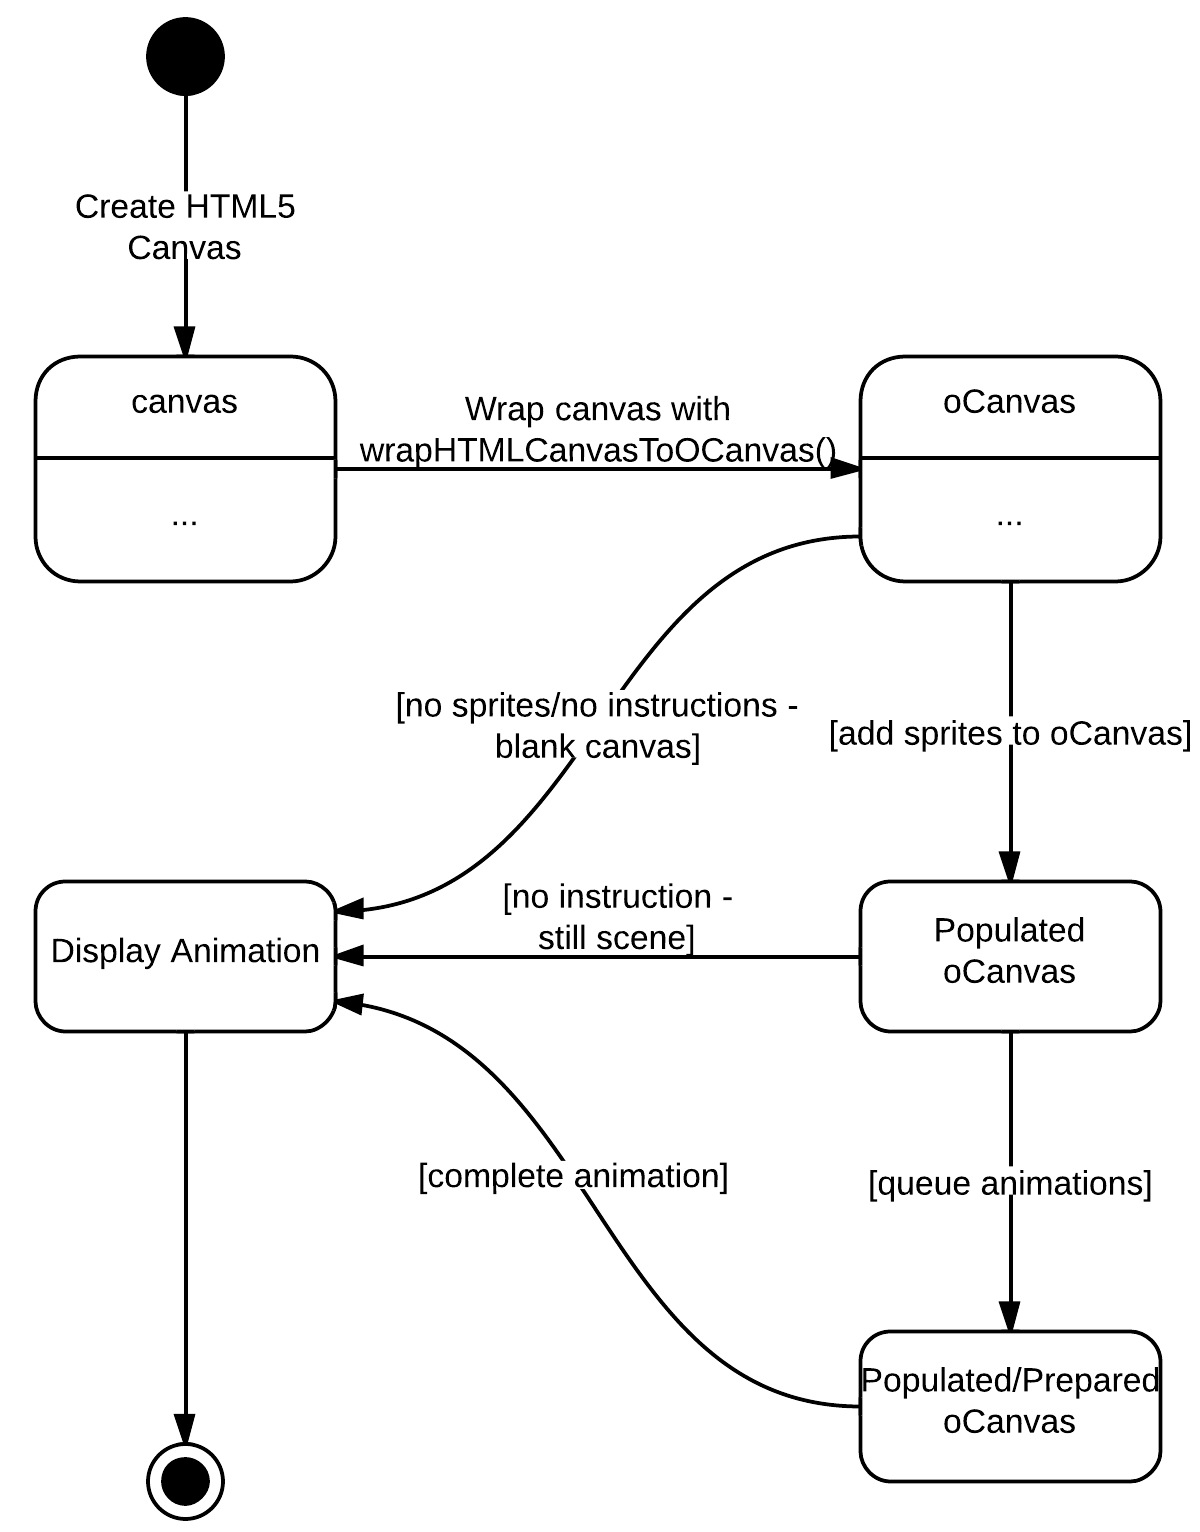
\includegraphics[scale=.3]{animation-statediagram.png}
    \caption*{After creating an HTML5 canvas user calls the wrapHTMLCanvasToOCanvas() to create oCanvas object. At this point sprites and instructions can be added to be displayed on the canvas object.}
\end{figure}
    

 \newpage
Our animation functions include a generic animate function and a series of pre-defined animations created by our group. The generic function is called move() and can animate a sprite in any combination of the x-axis, y-axis, and z-axis (rotation). This function is intended to be used for simple animations but also allows the flexibility for the programmer to call a series of move functions to create a more complex animation. Our pre-defined animations include jump, double jump, move left, move right, move up, and move down which can be called in addition to the generic move. The main content behind all of the animation functions is a animation block provided by the oCanvas library. This animation block allows for many optional parameters that can be used to produce different effects. Some of the effects that we utilized are easing functions, duration time, and animation queues. \\ 

\section{\emph{Individual Reflections}}
\subsection{Eric Lund}
\begin{changemargin}{1cm}{0cm} 
          Many challenges came up through development both technical and organizational throughout the whole development process. One of the biggest problems that stood out the most to me and falls in both the technical and organizational aspects was using GitHub for our source control.  The idea behind Git is awesome, and should make the development process much easier and efficient when working with a group of people but I felt that in our case it held us back. It was a technical problem in that none of the members in our group had really worked with Git, or even a true source source control system prior to this project. There were multiple times in the beginning of development in which we actually lost some work (nothing substantial, luckily) due to us not knowing the technical aspects of how Git/GitHub worked. Though the development process we gained a lot of experience with works Git and I think it ended up being a helpful tool — especially when we got to the integration periods with the other groups. The organizational challenge working with Git came by us not sufficiently managing our files in our branch. I was very hesitant (and I think I can speak for the team as well) in changing directories for files and moving folders around as it was only followed up by a series of merge conflicts and tracking problems. Because of that, our branch got messy real fast and wasn't as organized as it should of been. As a group it wasn't that big of a deal but if other groups wanted to look at what we had it would of been hard for them to find what they were looking for. \\
          
           Our group utilized many software engineering techniques during the development process but what stood out to me the most was our communication abilities. Our group had several meetings in which all of our members were able to attend and stay up to speed with the current development process. We even had several meetings that we didn't do any coding but rather talked about how we were going about on our implantation and what our next steps were going to be. Reflecting back this really made the whole process much easier.\\
           
           If I were to redo the whole process there are two things I would defiantly do. One of which would be to get a better grasp of Git/GitHub. I feel it would be beneficial if the whole group took time away from development to make sure we all knew and felt comfortable working with Git and also discuss as a group, how we would use it. Another thing I would do is communicate more with the other groups that directly affect what we are developing. As I said earlier, I felt the communication was exceptional in our group but it would of been even better if we extended that out to the other groups as well by staying updated on their current status and implementation. I had a great experience with my group members and felt like we accomplished the task at hand. 
\end{changemargin} 
\subsection{Kramer Canfield}
\begin{changemargin}{1cm}{0cm} 
KRAMER TYPES HERE
\end{changemargin} 
\subsection{Zeke Rosenberg}
\begin{changemargin}{1cm}{0cm} 
ZEKE TYPES HERE
\end{changemargin} 
\subsection{Calder Whiteley}
\begin{changemargin}{1cm}{0cm} 
CALDER TYPES HERE
\end{changemargin} 
\subsection{Jon Youmans}
\begin{changemargin}{1cm}{0cm} 
JON TYPES HERE
\end{changemargin} 


\section{\emph{Glossary} \& \emph{References}}
	
\end{document}
